\section{Community Evaluation: Empirical network}
\label{emp}
In this section, we demonstrate the performance of the \textbf{GN-$Q_M$} and \textbf{Louvain-$Q_M$} algorithms on the empirical dataset.
First we construct the multilayer networks based on the information extracted from the `Yelp' and `Meetup' datasets. Next, we explain 
the evaluation procedure and show that the proposed algorithms outperform the competing baselines.

\subsection{Yelp dataset}
% % We leverage on the dataset collected from Yelp\footnote{https://www.yelp.com/dataset\_challenge}, a popular location based social
% % network platform. First we describe
% % the Yelp dataset and explain the construction of the corresponding multilayer network. Next we describe the evaluation
% % procedure and demonstrate the performance of GN-$Q_M$ algorithm on the empirical dataset.

\subsubsection{Data description}
  The dataset obtained from Yelp~\cite{gupta2015complementary}, a popular location based social network (LBSN) platform,
  contains detailed information regarding Yelp
  customers/visitors (including their social connections \& residence),
  locations and the tips \& reviews posted by the customers. We assume that a customer $v$ visits a location $L$ if $v$ writes a
  tip/review for $L$.
  %For each location, the dataset contains information about its category (restaurants, hotels, shopping etc.),
  %latitude-longitude, address etc; similarly,
  %For each customer, we collect the details of her social connections, residence city etc. in the dataset.
%   Each location is indexed by
%   a \textit{location ID}, and contains information about its category (restaurants, hotels, shopping etc.),
%   latitude-longitude, address etc. as attributes.
%   Similarly, each visitor is indexed by \textit{a user ID} and contains information regarding her city, social connections etc.
%   The dataset contains information of total $61184$ business units located in $378$ cities and $366715$ customers during the
%   period $2005-2014$.
%   Each tip \& review entry is properly (daywise) timestamped and indexed by an unique \textit{tip/review id} containing the
%   corresponding visitor and business ID information.
%  Additionally, there are nearly 1.6 million reviews and 0.5 million tips in the dataset.
  We concentrate on the most popular city ``Las Vegas''
  containing $13,601$ locations and $173,697$ customers visiting those locations. To keep the network tractable, we first
  consider only the customers visiting locations within $5$KM radius from the center of the city. Then, we detect
  the maximally connected component in the friendship network of those visitors. This yields a set
  of $244$ connected customers. Furthermore, we consider only the $1627$ locations which are at least visited once by anyone of them.
  %[BM: Make it short. Perhaps we can only present the Las vegas data.]

\subsubsection{Construction of multilayer network $\mathcal{G}_{yelp}$}
%[BM:USE similar notation for synthetic network also, in the previous section]
We construct a multilayer network $\mathcal{G}_{yelp} =\{\{L_U, L_L\},\{L_{UL}\}\}$ for Yelp with two layers
where $L_U$ = ($V_U$, $E_U$) is the customer layer containing customer nodes and their social connections; $L_L$ = ($V_L$, $E_L$)
is the location layer containing location nodes and their proximity connections (any two locations within $200$ meters of each other are
connected)
and $L_{UL}$ = ($V_U$, $V_L$, $E_{UL}$) is the bipartite graph connecting customer node $c \in V_U$ with location node $l \in V_L$ if
customer $c$ visits the location $l$ (see Fig.~\ref{yelp}) .

% the bottom layer consists of
%  customers who are connected via social links and the top layer contains business nodes
%   where two businesses are connected
%   if and only if they are within ZZ meters of each other [BM:ZZ?]. We connect a customer node $v$  with a business node $B$ through a
%   coupling link if $v$ visits the business $B$ (see Fig.~\ref{yelp}). [BM: in this subsection, repeat the notations that
%   you introduced in representation section 2.]
  %The coupling link connecting a customer with a business node represents the visit of a customer to a business.

  %Finally, we add crosslayer (coupling) links between the nodes of this two layers with the help of
  %reviews i.e. we connect a visitor with a business if she has written at least one review for that business (see Fig.~\ref{yelp}).
\begin{figure}
\begin{center}

\subfigure[\vspace{-0.22in}Precision
]{\label{reco1}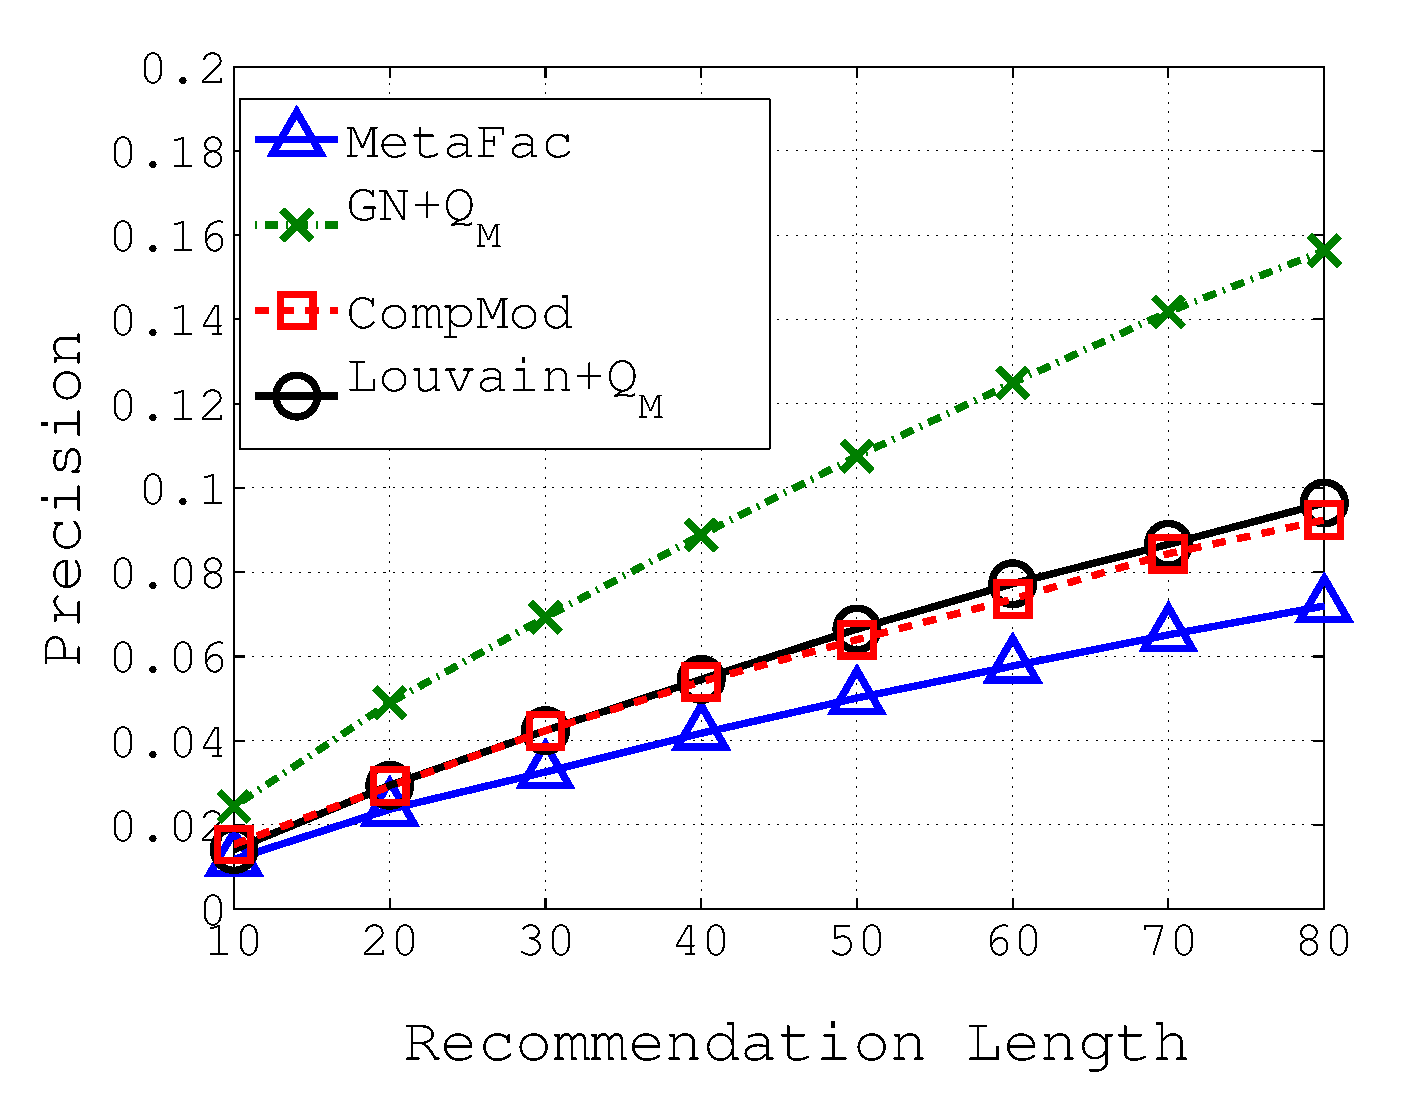
\includegraphics[angle=0,scale=.18]{./images/Intersection_Reco_march21_square_new.pdf}}
\subfigure[\vspace{-0.22in}F1 Score
]{\label{reco0}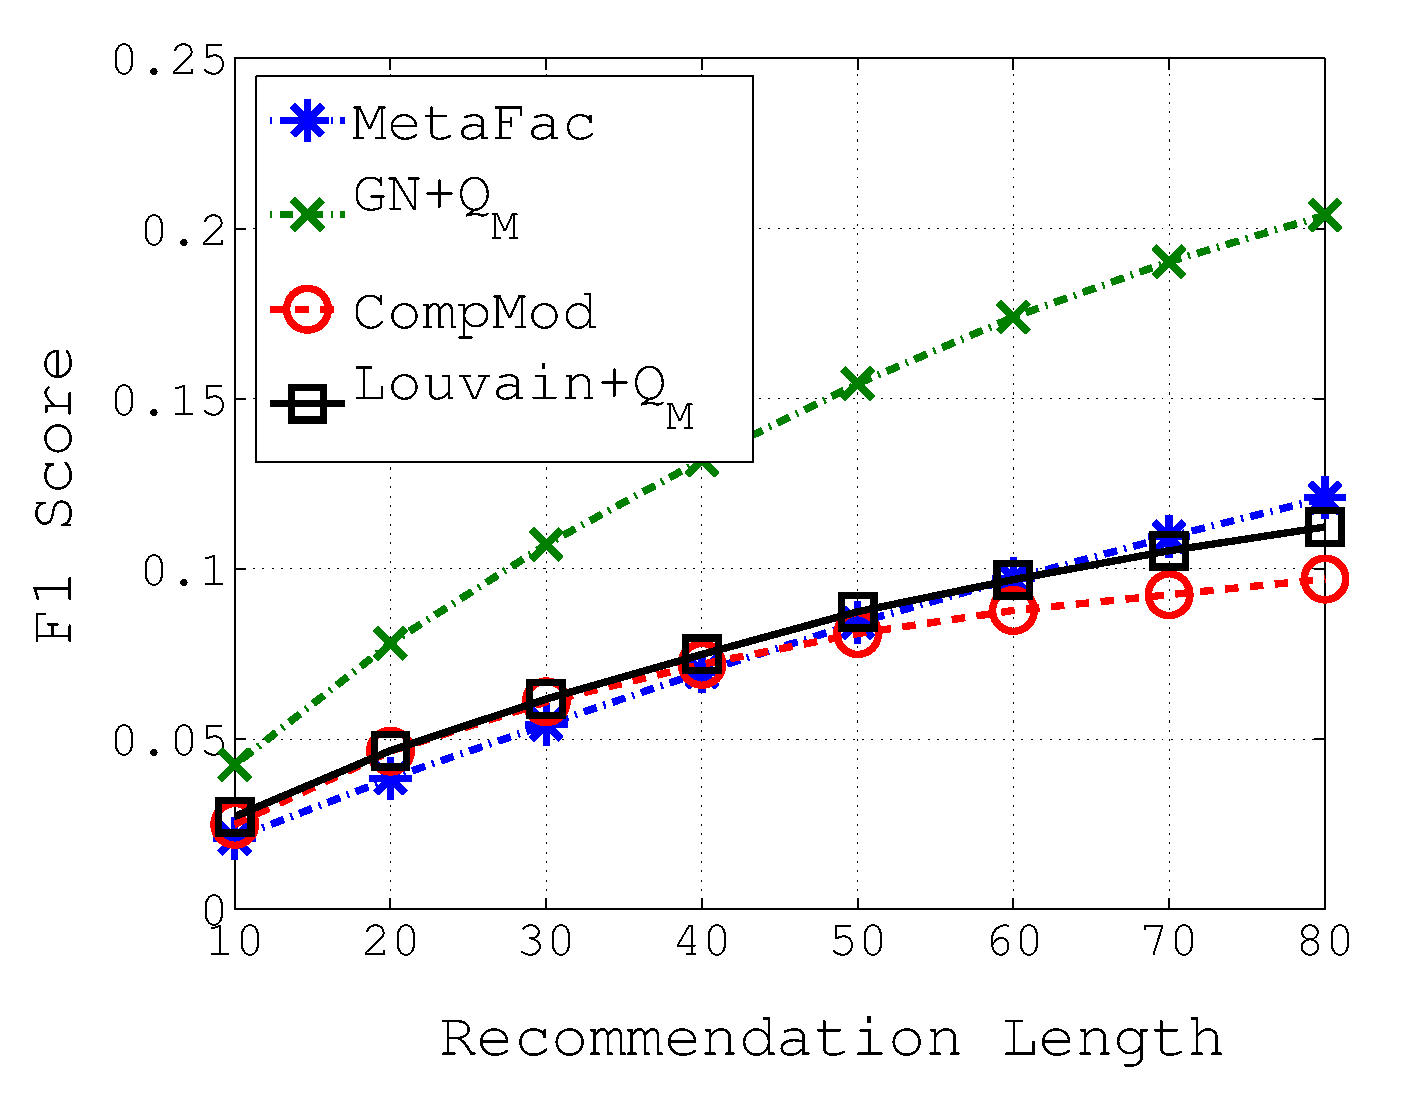
\includegraphics[angle=0,scale=.18]{./images/F1_Reco_march21_square_new.pdf}}
\end{center}
\vspace{-0.25in}
\caption{Precision \& F1 Score (avg. over all visitors) for communities obtained from different algorithms 
for various recommendation lengths on Yelp N/W.}
\vspace{-0.25in}
\label{reco}
\end{figure}





\subsubsection{Evaluation procedure}
%[BM: use suitable notations from section 2]
Unlike synthetic dataset, obtaining ground truth communities for the empirical network is challenging.
We evaluate the performance of the community detection algorithms on this network indirectly using a location recommendation framework.
In the LBSN platform, location recommendation is a standard problem~\cite{gupta2015complementary} where for one visitor $v \in V_U$, a
set of potential
locations $L \subseteq V_L$ are recommended for her future visit, based on the interest profile of $v$.
First, we apply location similarity based collaborative filtering~\cite{resnick1994grouplens} on the empirical dataset to obtain a set
of $K$ recommended locations for each visitor $v$ and consider it as our ground truth.
% Collaborative filtering basically estimates the pair wise location
% similarities utilizing their visitor overlap and then recommends each user $v$ a set of locations similar to ones she
%has already visited.
%We consider this per visitor location recommendation as ground truth.
Next, we apply the multilayer community detection algorithms on $\mathcal{G}_{yelp}$ and obtain $K'$ disjoint
communities $C_1, C_2,\dots,C_{K'}$. As explained in section~\ref{dataset}, each $C_i$ can be expressed as
$\{\{L^{C_i}_U, L^{C_i}_L\},\{L^{C_i}_{UL}\}\}$ where $L^{C_i}_U = (V^{C_i}_U, E^{C_i}_U)$,
$L^{C_i}_L = (V^{C_i}_L, E^{C_i}_L)$ and $L^{C_i}_{UL}$ = ($V^{C_i}_U$, $V^{C_i}_L$, $E^{C_i}_{UL})$.
% we extract the set of unvisited location
% nodes $L \subseteq V_L$ which is a member of the community $C_i$. %[BM: use proper notations].
We claim that for a visitor $v \in V^{C_i}_U$, the set $V^{C_i}_L$ is the recommended locations to visit,
following the community detection algorithms.
We evaluate this set $V^{C_i}_L$ against collaborative filtering based ground truth.

\subsubsection{Evaluation metrics \& Performance}
%[BM: use f1-score and precision]
Suppose, for a visitor $v$, $L_C$ is the set of locations recommended by the multilayer community detection algorithms and
 $L_R$ is the set of locations recommended by collaborative filtering. In such a scenario, we calculate the (a) Precision
 and (b) F1 Score of the recommendations as $\frac{\left\vert L_C \cap L_R \right\vert}{\left\vert L_C \right\vert}$ and
 $\frac{2 \left\vert L_C \cap L_R \right\vert}{\left\vert L_C \right\vert + \left\vert L_R \right\vert}$
 respectively. Notably, we do not use Recall ($\frac{\left\vert L_C \cap L_R \right\vert}{\left\vert L_R \right\vert}$) here to avoid bias 
 towards large communities.
% %  
% %  \footnote{Similarly, we can also define recall of the detected communities
% %  as $\frac{\left\vert L_C \cap L_R \right\vert}{\left\vert L_R \right\vert}$. But, we do not use it as it introduces bias towards
% %  algorithms detecting larger communities.}.
%  (a) Precision:  In that case, precision of the detected communities
%  can be measured as .
%  %between this two sets i.e. $J_{Sim} = \frac{\left\vert L_C \cap L_R \right\vert}{\left\vert L_C \cup L_R \right\vert}$.
%
%  (b) F1 Score: This can be calculated as
In Fig.~\ref{reco}, we plot precision and F1 score (averaged over all visitors) with varying recommendation length $K$ for our algorithms 
along
with the state of the art competing algorithms. Increasing $K$ usually increases the
numerator ($\left\vert L_C \cap L_R \right\vert$) for both the
metrics, resulting in an increasing pattern of precision and F1 score.
Clearly, both \textbf{GN-$Q_M$} \& \textbf{Louvain-$Q_M$} (especially, \textbf{GN-$Q_M$}) outperforms the competing algorithms for
almost all $K$ values, demonstrating the elegance of the proposed algorithms.


\begin{figure}
\centering
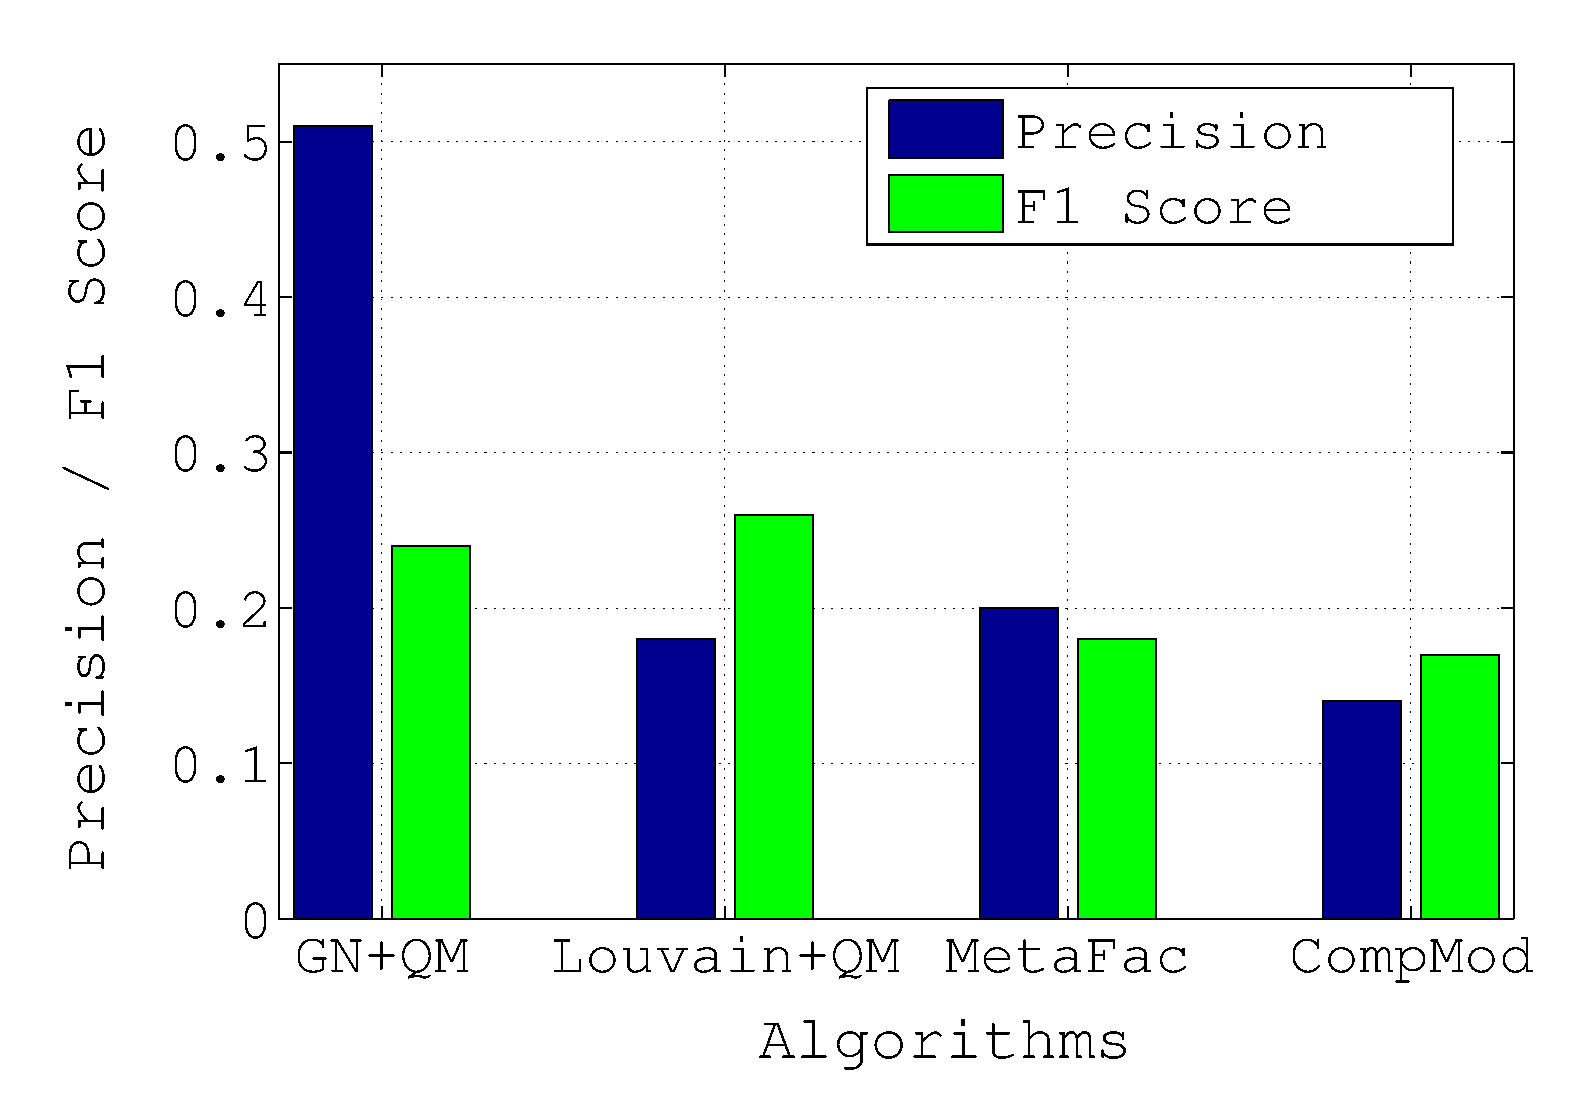
\includegraphics[width=2in]{./images/Meetup_precision_no_mq.pdf}
\vspace{-0.2in}
\caption{Precision \& F1 Score (averaged over all groups) for communities obtained from different algorithms on Meetup N/W.}
\vspace{-0.2in}
\label{meetup}
\end{figure}

\subsection{Meetup dataset}
% Meetup is a popular event based social networking (EBSN) portal that facilitates
% hosting events in various localities around the world.
% We develop a crawler to collect the Meetup data\footnote{\url{https://www.meetup.com/meetup_api/}} for the city of Chicago
% during a period of 20 months (from August 2015 to March 2017).
% In the following, we first describe
% the crawled dataset and explain the construction of the corresponding multilayer network. Next, we describe the evaluation
% procedure and demonstrate the performance of GN-$Q_M$ \& Louvain-$Q_M$ algorithms on this empirical dataset.

\subsubsection{Data description}
Meetup, a popular event based social networking (EBSN) platform, facilitates similar minded people to form online groups and
organize offline events.
We develop a crawler to collect the Meetup~\cite{pramanik2016predicting}
%({\url{https://www.meetup.com/meetup_api/}}) 
data for the city Chicago
during a period of 20 months (from August 2015 to March 2017).
The crawled dataset contains the details of $5727$ Meetup groups, $342,773$ members and $31,719$ events hosted
by those groups. The dataset contains the exact time, when a Meetup user joins a specific Meetup group.
Additionally, we collect the profile for each Meetup group and its members which are characterized by suite of predefined tags 
($20$ tags for members; $56$ for groups)
such as `web design', `foodie', `cycling' etc. reflecting
their respective preferences. In order to keep the network tractable, first we filter out all the Meetup groups possessing more than
$30$ members. Next, we select only the groups having at least $10$ members joined before the ${30}^{th}$ 
November, 2016 (i.e. within the first $80\%$ of the crawling period) and
at least $5$ members joining in next $4$ months (last $20\%$ of the crawling period). Finally, we obtain $49$ Meetup groups and their 
corresponding $1194$ members.
%  From the $5727$ groups present in the dataset,
%   we focus on the most popular city ``Las Vegas''
%   which contains $13601$ locations and $173697$ users visiting those locations. To reduce the size of the network, we first
%   consider only the users visiting locations within $5$KM radius from the center of the city. Then, we detect
%   the maximally connected component in the friendship network of those visitors. This yields a set
%   of $244$ connected users. Furthermore, we consider only the $1627$ locations which are at least visited once by anyone of them.
  %[BM: Make it short. Perhaps we can only present the Las vegas data.]

\subsubsection{Construction of multilayer network $\mathcal{G}_{meetup}$}
%[BM:USE similar notation for synthetic network also, in the previous section]
We construct a multilayer network $\mathcal{G}_{meetup} =\{\{L_M, L_G\},\{L_{MG}\}\}$ containing all groups and members
%from Meetup dataset
collected during the
%first $80\%$ of the
entire crawling period.
%(till ${31}^{st}$ of March, 2017, denoted as training period).
The network contains the following two layers; $L_M$ = ($V_M$, $E_M$) is the member layer containing user nodes and their similarity based
connections and $L_G$ = ($V_G$, $E_G$) denotes the group layer containing Meetup groups as nodes and their respective similarity based 
connections.
In both the layers, similarities between node pairs are computed based on the Jaccard coefficient of their respective tags overlap;
we connect
the top $33^{rd}$ percentile of node pairs in $L_M$ \& $L_G$.
$L_{MG}$ = ($V_M$, $V_G$, $E_{MG}$) is the bipartite graph connecting a member node $x\in V_M$ with a group node $g \in V_G$ if $x$ is
a member of Meetup group $g$ before November 30, 2016.

% the bottom layer consists of
%  customers who are connected via social links and the top layer contains business nodes
%   where two businesses are connected
%   if and only if they are within ZZ meters of each other [BM:ZZ?]. We connect a customer node $v$  with a business node $B$ through a
%   coupling link if $v$ visits the business $B$ (see Fig.~\ref{yelp}). [BM: in this subsection, repeat the notations that
%   you introduced in representation section 2.]
  %The coupling link connecting a customer with a business node represents the visit of a customer to a business.

  %Finally, we add crosslayer (coupling) links between the nodes of this two layers with the help of
  %reviews i.e. we connect a visitor with a business if she has written at least one review for that business (see Fig.~\ref{yelp}).


\subsubsection{Evaluation procedure}
%[BM: use suitable notations from section 2]
%Unlike synthetic dataset, obtaining ground truth communities for the empirical network is non trivial.
We evaluate the performance of the community detection algorithms with the help of a group recommendation framework.
In the EBSN platform, recommending suitable groups to Meetup users is a well studied problem~\cite{group_reco2_TASP}, where for 
user $x$, a set of groups $g_S \subseteq V_G$
are recommended.
% % We evaluate the performance of the community detection algorithms with the help of a group recommendation framework,
% % a well studied problem~\cite{group_reco2_TASP}
% % in the EBSN platform, 
% % %recommending suitable groups to Meetup users is a well studied problem~\cite{group_reco2_TASP}, 
% % where for user $x$, a set of suitable groups $g_S \subseteq V_G$ are recommended.
% In oure apply location similarity based collaborative filtering~\cite{resnick1994grouplens} on the empirical dataset to obtain a set
% of $K$ recommended locations for each visitor $v$ and consider it as our ground truth.
% Collaborative filtering basically estimates the pair wise location
% similarities utilizing their visitor overlap and then recommends each user $v$ a set of locations similar to ones she
%has already visited.
%We consider this per visitor location recommendation as ground truth.
To perform the same, we first apply the multilayer community detection algorithms on $\mathcal{G}_{meetup}$ and obtain $K$ disjoint
communities $C_1, C_2,\dots,C_K$. As explained in section~\ref{dataset}, each $C_i$ can be expressed as
$\{\{L^{C_i}_M, L^{C_i}_G\},\{L^{C_i}_{MG}\}\}$ where $L^{C_i}_M = (V^{C_i}_M, E^{C_i}_M)$,
$L^{C_i}_G = (V^{C_i}_G, E^{C_i}_G)$ and $L^{C_i}_{MG}$ = ($V^{C_i}_M$, $V^{C_i}_G$, $E^{C_i}_{MG})$.
% we extract the set of unvisited location
% nodes $L \subseteq V_L$ which is a member of the community $C_i$. %[BM: use proper notations].
Suppose, for a group $g \in V_G$, we define ${B}_g \subseteq V_M$ and ${A}_g \subseteq V_M$ as the set of members joining $g$
during the training (before Nov. $30$) and test period (after Nov. $30$) respectively.
We claim that for a group $g \in V^{C_i}_G$, $(V^{C_i}_M-{B}_g)$ is the set of users recommended to join the Meetup group $g$ in the 
test period.
%We evaluate this set $(V^{C_i}_M-{B}_g)$ against the actual set of users ${A}_g$ joining the group $g$ after ${31}^{st}$ of November, 2016.

\subsubsection{Evaluation metrics \& Performance}
%[BM: use f1-score and precision]
 Following the aforesaid procedure, let $M_g$ be the set of recommended users (by the community detection algorithms),
 to join the Meetup group $g$ in the test period. ${A}_g$ provides the ground truth information of group membership in the test 
 period. Hence, we calculate the (a) Precision and (b) F1 Score of the recommendation
 as $\frac{\left\vert M_g \cap A_g \right\vert}{\left\vert M_g \right\vert}$ and
 $\frac{2 \left\vert M_g \cap A_g \right\vert}{\left\vert M_g \right\vert + \left\vert A_g \right\vert}$
 respectively.
%  \footnote{We do not use Recall ($\frac{\left\vert M_g \cap A_g \right\vert}{\left\vert A_g \right\vert}$) to avoid bias 
%  towards large 
%  communities.}.
% %  \footnote{Similarly, we can also define recall of the detected communities
% %  as $(\left\vert M_g \cap A_g \right\vert)/(\left\vert A_g \right\vert)$. But, we do not use it as it introduces bias towards
% %  algorithms detecting larger communities.}.
%  {Similar to Yelp, here also we do not use recall
%  ($\frac{\left\vert M_g \cap A_g \right\vert}{\left\vert A_g \right\vert}$) due to its bias towards
%  algorithms detecting larger communities.}.
%  (a) Precision:  In that case, precision of the detected communities
%  can be measured as .
%  %between this two sets i.e. $J_{Sim} = \frac{\left\vert L_C \cap L_R \right\vert}{\left\vert L_C \cup L_R \right\vert}$.
%
%  (b) F1 Score: This can be calculated as
In Fig.~\ref{meetup}, we plot the precision and F1 score (averaged over all groups) for proposed algorithms against the competing algorithms.
Evidently, \textbf{GN-$Q_M$} outperforms the competing algorithms in terms of precision whereas \textbf{Louvain-$Q_M$} performs the best
in terms of F1
score, demonstrating the elegance of our proposed algorithms for the Meetup dataset.

%
% \begin{figure}
% \centering
% 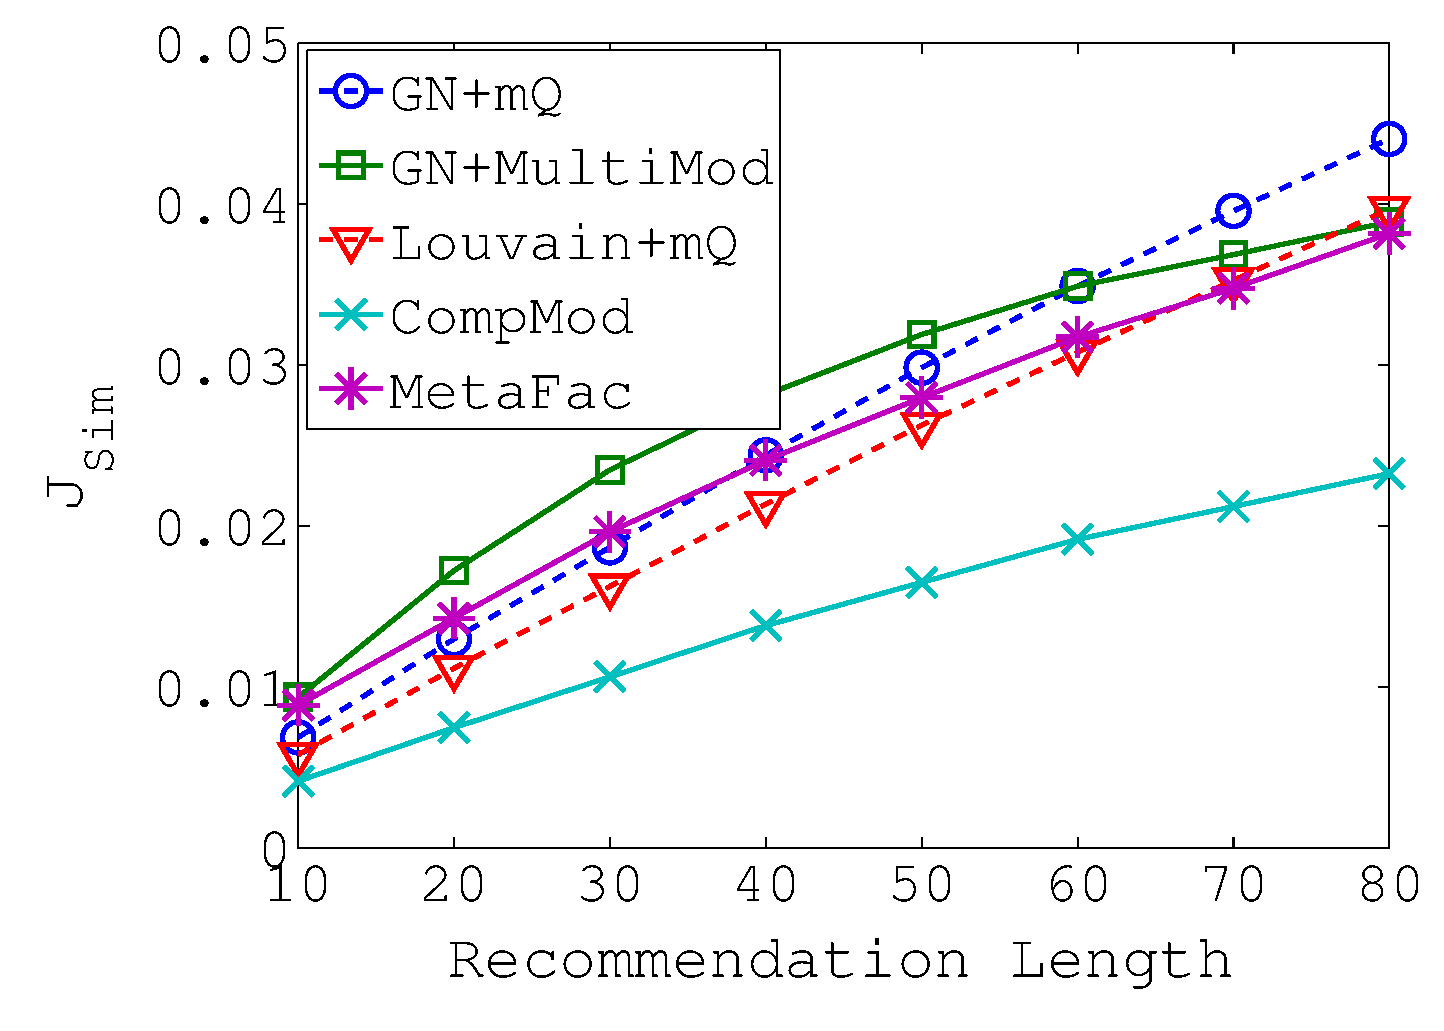
\includegraphics[width=3.5in]{./images/Jaccard_Reco.pdf}
% \vspace{-0.1in}
% \caption{$J_{Sim}$ for communities obtained from different algorithms for various recommendation length}
% \vspace{-0.1in}
% \label{reco1}
% \end{figure}
%
% \begin{figure}
% \centering
% 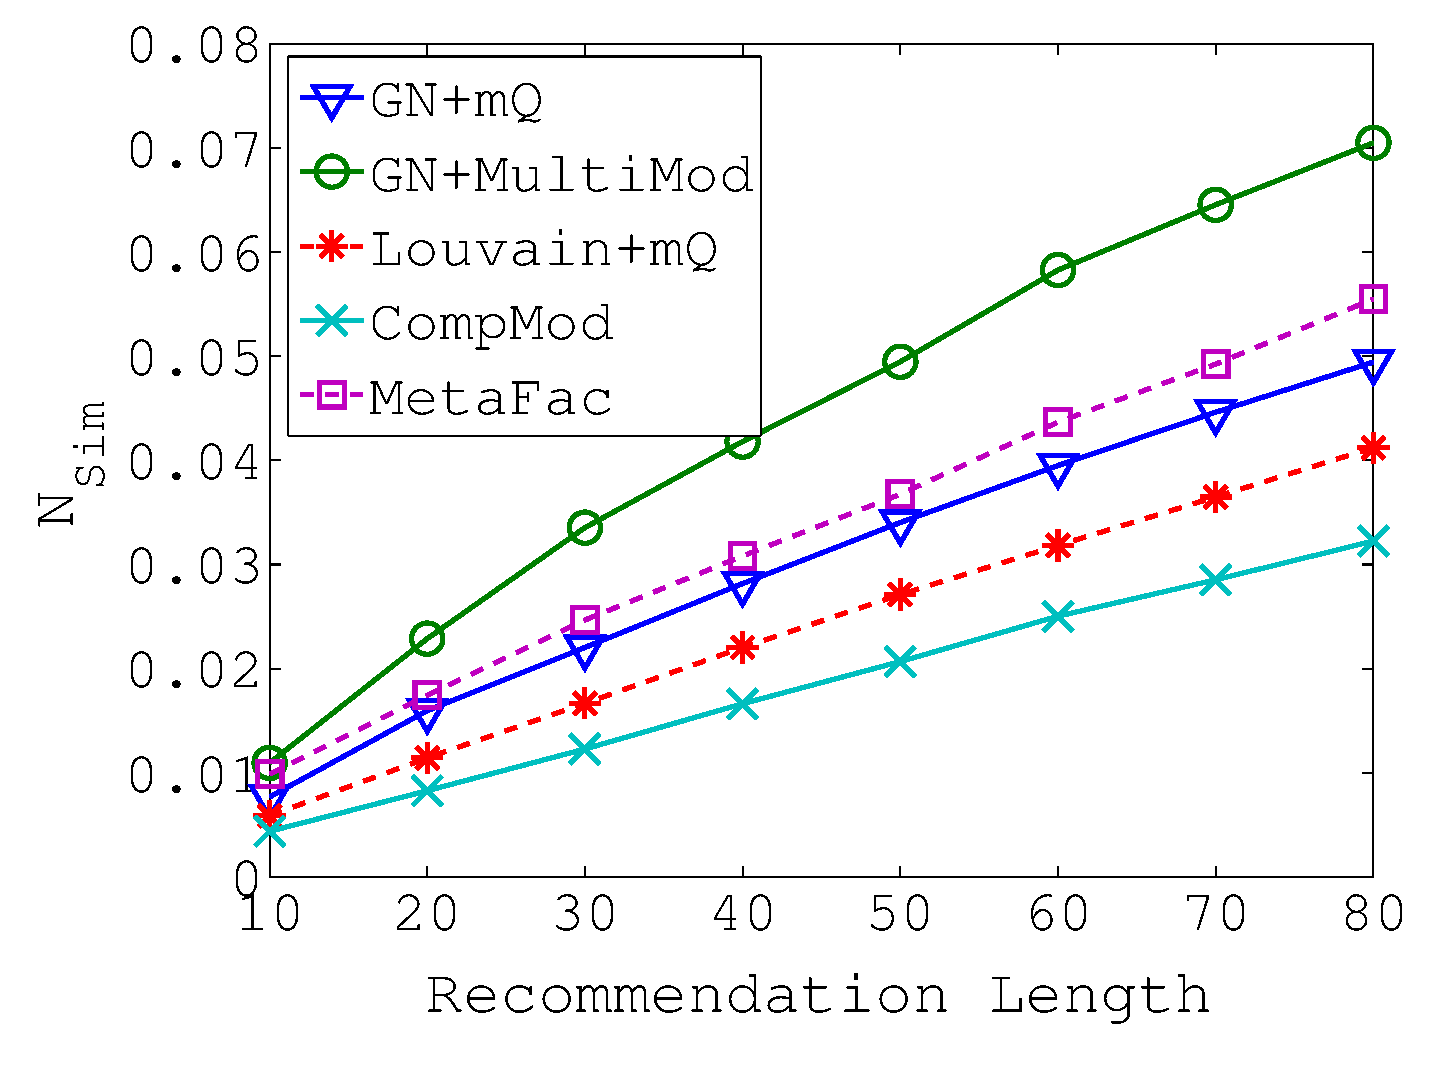
\includegraphics[width=3.5in]{./images/Intersection_Reco.pdf}
% \vspace{-0.1in}
% \caption{$N_{Sim}$ for communities obtained from different algorithms for various recommendation length}
% \vspace{-0.1in}
% \label{reco2}
% \end{figure}
% [BM: drop if necessary]
% \subsection{Scalability \& Adaptability}
% In this subsection, we discuss how scalable our algorithm is and how it can adapt if the network becomes more complicated.
%
% \subsubsection{Scalability:}
% Scalability of community detection algorithms has always been an issue. Here, we categorically surpass this problem by using
% scalable single layer community detection algorithms like Louvain~\cite{blondel2008fast} and
% Girvan-Newman~\cite{newman2004fast}, as our base algorithms to optimize $Q_M$.
% As this algorithms are already proven to be scalable, there is no such scalability issue for our approach.
%
% \subsubsection{Adaptability:}
% In this paper, we show all the results with respect to 2-layer networks for the ease of understanding and representation. Nevertheless, our
% approach can be easily extended for networks with higher number of layers by modifying the $Q_M$ definition trivially. For example, if we
% wish to detect communities in a 3-layer network containing two bipartite coupling layers, there will be five terms in
% $Q_M$ - three single layer modularity terms and two bipartite modularity terms. 